\section{导体和绝缘体}\label{sec:7-3}

电线里面的芯都是金属丝,在金属丝的外面还要包上一层橡皮或者塑料,这是为什么呢?
为了说明这个问题,我们来做个实验。

\begin{figure}[htbp]
    \centering
    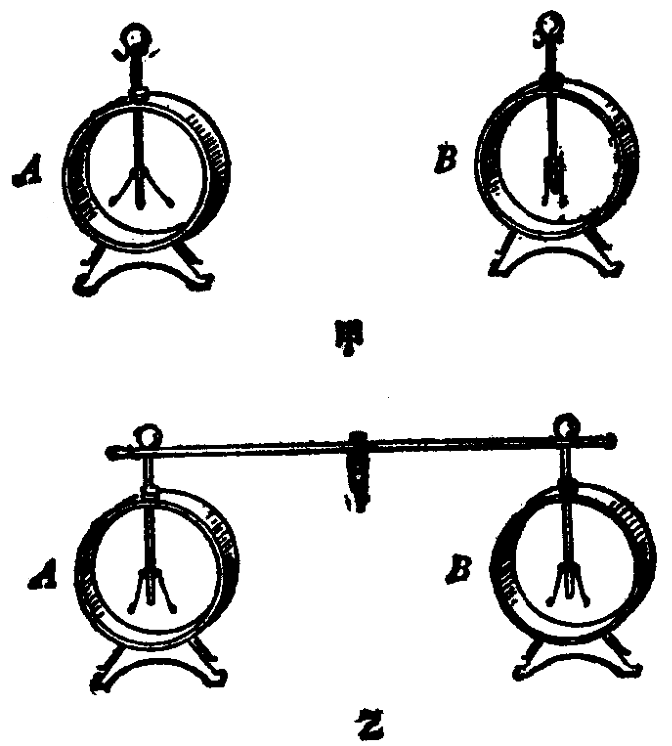
\includegraphics[width=0.6\textwidth]{../pic/czwl2-ch7-8}
    \caption{}\label{fig:7-8}
\end{figure}

取两个相同的验电器 $A$、$B$,使 $A$ 带电,$B$ 不带电(图 \ref{fig:7-8} 甲)。
拿一根带橡胶柄的金属棒,把这两个验电器连接起来,可以看到,
$B$ 的金属箔张开了,同时 $A$ 的金属箔张开的角度减小了(图 \ref{fig:7-8} 乙)。
这表示 $A$ 上的一部分电荷通过金属棒传到 $B$ 上去了。
如果不用金属棒,而用玻璃棒或橡胶棒来连接 $A$ 和 $B$,$B$ 的金属箔就不张开。
这表示 $A$ 上的电荷不能够通过玻璃棒或橡胶棒传到 $B$ 上去。

上面的实验表明,有的物体容易导电,有的物体不容易导电。

容易导电的物体叫做\textbf{导体}。金属、人体、大地以及各种酸、碱、盐的水溶液都是导体。

不容易导电的物体叫做\textbf{绝缘体}。橡胶、塑料、玻璃、陶瓷、油、空气都是好的绝缘体。

为什么导体能够导电,绝缘体不能够导电呢?
原来,导体中有能够自由移动的电荷,因此在导体里电荷能够从一个地方传到别的地方。
绝缘体中的电荷几乎都被束缚在原子或分子的范围内,不能自由移动,因此在绝缘体里电荷不能从一个地方传到别的地方。
金属是最重要的导体,在金属里能够自由移动的电荷就是电子,这种能自由移动的电子叫做\textbf{自由电子}。
在酸、碱、盐的水溶液里,能够自由移动的电荷是正离子和负离子。

好的导体和好的绝缘体都是重要的电工材料,在技术上应用很广。
电线芯用金属来做,是因为金属是导体,能够导电;
外面包上一层橡皮或者塑料,是因为这些材料是绝缘体,能防止漏电或触电。
许多电学仪器,有的部分需要用导体来做,有的部分又需要用绝缘体来做。

导体和绝缘体并没有绝对的界线,在通常情况下是很好的绝缘体,当条件改变时也可能变成导体。
例如,如果用一根干木棒把图 \ref{fig:7-8} 中的两个验电器连起来,会看到干木棒不导电。
把这根木棒弄湿,会看到湿木棒导电了。这表明,绝缘体潮湿了会导电。
因此,电器的绝缘部分要保持干燥,以免漏电和发生触电事故。

除了导体和绝缘体,还有一类物体,它们的导电能力在导体和绝缘体之间,叫做半导体。
由于半导体有许多独特而有用的性质,因而在电子技术和无线电技术中有着广泛的应用。


\lianxi

\begin{wrapfigure}[10]{r}{7cm}
    \centering
    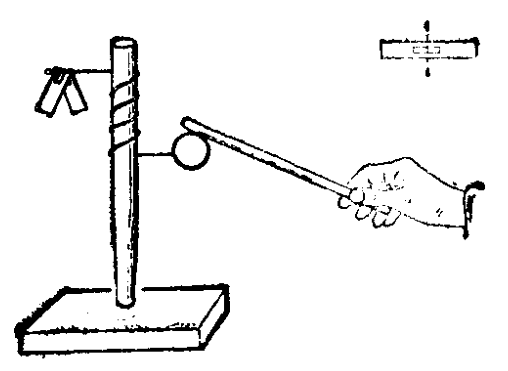
\includegraphics[width=6cm]{../pic/czwl2-ch7-9}
    \caption{自制的简单验电器}\label{fig:7-9}
\end{wrapfigure}

(1) 为什么用摩擦的方法可以使拿在手中的胶木棒带电,却不能使拿在手中的金属棒带电?
怎样才能使拿在手中的金属棒带电?

(2) 电工修电路的时候,使用有木柄或者柄上套着橡胶套的工具,并且常常站在干燥的木凳上,为什么?

(3) 观察一下验电器,看看它的哪些部分是导体,哪些部分是绝缘体?

(4) 在图 \ref{fig:7-4} 中,为什么带电体接触验电器金属棒上端的金属球,金属棒下端的两条金属箔就会张开?

(5) 照图 \ref{fig:7-9} 那样,把塑料笔杆插在座子上(座子可以用橡皮泥或泥土来做),在笔杆上缠一段金属丝。
金属丝的左端挂一条对折的金属箔(可以用包纸烟的金属箔照图 \ref{fig:7-9} 右上角画的那样剪好沿虚线对折),
金属丝的右端绕成环状,这样就做成了一个简单的验电器。
当带电体接触右边的金属环时,左边的金属箔就张开,为什么?
自己做一个简单的验电器,并且用它检验跟头发摩擦过的塑料梳子带不带电。

